\section{Discussion}

The RMSE values in Table~\ref{tab:rmse} and the visual comparisons reveal clear differences in the stability and reliability of the interpolation methods for summer 2-meter air temperature at 10 AM in Iran. While all four approaches can reconstruct the general trend of temperature within the training range, their performance diverges significantly when the training interval is changed or when extrapolation is required \cite{atkinson1989introduction, burden2011numerical, smith2020numerical, brown2021polynomial, garcia2022newton}.

Local Newton Forward and Backward methods, although capable of fitting the data well within the training interval, are highly sensitive to the choice of training range. Their RMSE increases dramatically when the interval is shifted, and visual inspection shows that error accumulation (error propagation) is a major issue—especially near the boundaries and outside the training window. This accumulation of error is a hallmark of classical polynomial interpolation, where small inaccuracies at each step can quickly amplify, leading to instability and unreliable predictions \cite{lee2019comparison, press2007numerical}.

Local Lagrange interpolation, while sometimes providing high accuracy in dense regions, suffers even more from error accumulation and Runge's phenomenon, as reflected in its extremely large RMSE values when the training interval does not cover the full prediction range. This method is particularly vulnerable to instability when used for extrapolation or with non-uniform data \cite{smith2020numerical}.

In contrast, Local Polynomial Regression stands out as the most robust and stable method. Its RMSE remains low even when the training interval is restricted, and its predictions are less affected by error accumulation. This method effectively balances flexibility and noise reduction, making it the most reliable choice for both interpolation and limited extrapolation in regional temperature analysis \cite{brown2021polynomial}.

Given the superior stability and generalization of local polynomial regression, we used this method to forecast the 2-meter air temperature at 10 AM for the upcoming decade (the 2020s) in Iran. The model was trained on the full interval [1950, 2020] and then used to predict values for 2021--2030. Figure~\ref{fig:future-prediction} shows the extrapolated results. While such forecasts can provide valuable insights into potential future trends, it is important to interpret them with caution, as uncertainty grows rapidly outside the observed data range and unforeseen climate events or nonlinearities may not be captured by the model.

\begin{figure}[htbp]
    \centering
    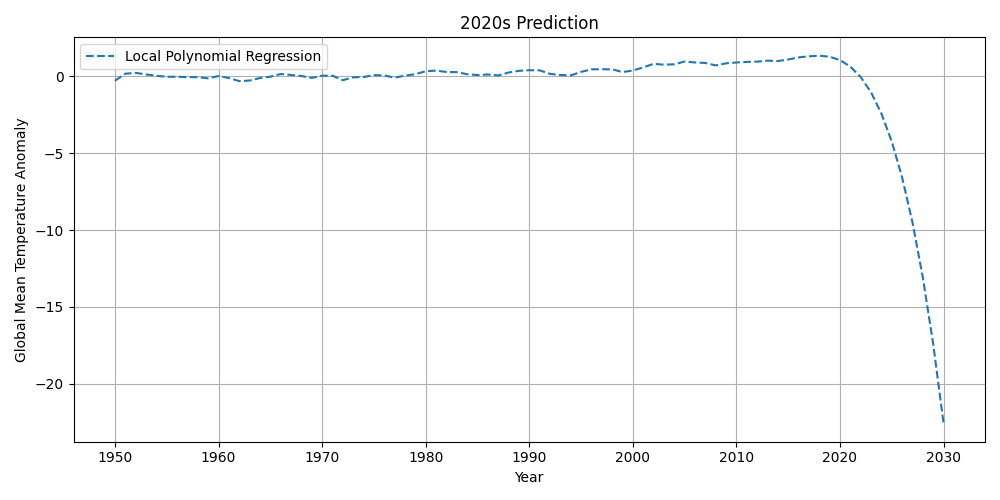
\includegraphics[width=0.8\textwidth]{../figs/2020s-prediction.png}
    \caption{Local Polynomial Regression prediction of 2-meter air temperature at 10 AM for 2021--2030 in Iran, trained on [1950, 2020] using ERA5-Land \cite{ERA5}.}
    \label{fig:future-prediction}
\end{figure}

Additional practical steps, such as data cleaning, normalization within local windows, and robust fallback to linear interpolation, further enhance the reliability and interpretability of the results \cite{burden2011numerical}.